\documentclass[12]{amsart}

\usepackage{amssymb,amsmath}

%\usepackage{refcheck}

\newtheorem{theorem}{Theorem}[section]
\usepackage{graphicx}
\usepackage{amssymb}
\usepackage{mathrsfs}
\usepackage{amsmath}
\usepackage{latexsym}
\usepackage{amssymb}
\usepackage{enumerate}
\usepackage{fullpage} 
\usepackage{setspace}
\usepackage{color}
\usepackage{ dsfont }
\usepackage{float}
\usepackage{physics}

\doublespacing
\title[CS590 Computer Security Final Project]{Implementing the BB84 Protocol Using IBM's Q Simulator}
\author{Faris Sbahi}
\author{Kya Sorli}
\author{Samantha Washko}
\begin{document}
\maketitle

\section{Introduction}

Quantum computing and its derivatives are some of the most exciting new areas of computer science, and have special relevance for the realm of computer security. Though quantum computing has several remarkable applications, including the potential to break sophisticated public-key cryptosystems like RSA\cite{text}, in this paper we will focus on a more defensive use:  quantum cryptography. Also known as quantum key distribution, quantum cryptography is a procedure that guarantees unconditional security \cite{challenge} by taking advantages of fundamental quantum mechanical properties in an effort to provide a secure method of exchanging information\cite{text}. Peter Shor, the developer of Shor's algorithm, and John Preskill describe the difference between conventional and quantum cryptography as centering around the fact that in quantum cryptography, "The data are kept secret by the properties of quantum mechanics, rather than the conjectured difficulty of computing certain functions."\cite{bb84}

Furthermore, one can use coherent information, a measure of quantum information, to give an "information-theoretic lower bound" on the ability to send private information over quantum communication channel. As a result, quantum information may have special relevance to quantum cryptography in that it can prove the security of quantum key distribution protocols \cite{text}.

At present, quantum cryptography is still a new and relatively untested field, but it has already begun to be deployed in the commercial and defense realms\cite{sat}\cite{challenge}. IBM is one of the companies that has been at the forefront of such implementations. At the present, they offer cloud quantum computers and simulators that range from 5 to 32 qubits. Even though this is a powerful tool, there are no demos of QKD currently available using this, or any real quantum simulator.

Accordingly, in this paper. we aim to implement the well-known quantum key distribution protocol, BB84, and run it on the IBM Q Simulator. We also seek to demonstrate its unconditional security by means of proof and empirical evidence.

\section{Background}

To provide context, this section will endeavor to discuss the background information for three concepts central to the experiment performed in this paper. This will include descriptions of Quantum Key Distribution (QKD), the BB84 Protocol, and information reconciliation and privacy amplification. 

\subsection{Quantum Key Distribution}
As stated previously, one of the primary motivations for quantum cryptography is to address the need for secure communication of information, such as private keys used in private or public-private key cryptosystems. Although methods such as Diffie-Hellman 
\cite{DH} already exist for this purpose, they are limited. With Diffie-Hellman, for example, it is difficult to detect man-in-the-middle attacks or eavesdropping. Quantum cryptography and quantum key distribution (QKD), seeks to remedy this directly.

QKD is a \textit{provably secure} protocol that allows for the creation of private key bits between two parties over a public channel. The resulting key bits are then used to implement a "classical private key cryptosystem" that allows for secure communication between the parties\cite{text}. The central pillar of QKD is its ability to reveal the presence of eavesdroppers. At a high level, the QKD protocol requires a that qubits be "communicated over the public channel with error rate lower than a certain threshold"\cite{text}, a requirement that would not hold true if eavesdroppers had compromised the security of the message.

QKD accomplishes security by exploiting the properties of quantum mechanics and information. Due to these properties, measuring the qubits in a message inherently disturbs their state. Consider two parties, Alice and Bob, and a potential eavesdropper Eve. When Alice attempts to send information to Bob, it is impossible for Eve to access and learn the information without disturbing the state of the qubits in Alice's message. As a result, Alice and Bob would be able to tell that someone was listening in on their correspondence\cite{text}.

This simplifies to a central proposition: any attempt to gain information results in state disturbance. When trying to distinguish between "two non-orthogonal quantum states, information gain is only possible at the expense of introducing disturbance to the signal"\cite{text}. For a proof of this proposition, please see pages 586-7 of Nielson \& Chuang's \textit{Quantum Computation and Quantum Information} text.

The steps used to detect an eavesdropper using QKD can be condensed to the following\cite{text}:

\begin{enumerate}
\item Transmit non-orthogonal qubits between Alice and Bob. 
\item Check for disturbances in the transmitted states to establish an upper bound on noise or eavesdropping.
\item \textit{Check} qubits are interspersed regularly among data qubits. The noise limit applies to these qubits as well as the data. 
\item Alice and Bob perform information reconciliation and privacy amplification (Discussed in the following section) to get the shared secret key.
\item The threshold max error rate is determined by the efficacy of best information reconciliation and privacy amplification protocols.

\end{enumerate}

\subsection{The BB84 Protocol}\label{bb84}

The BB84 protocol is a specific QKD protocol that was developed by C. H. Brennett and G. Brassard in 1984\cite{bb84}. It was the first QKD protocol proposed and is the most widely deployed protocol\cite{sat}\cite{bb84}.

In this paper, we sought to implement the BB84 protocol on the IBM Q-Simulator. The steps undergone during BB84 are explained in \cite{text}, but are reproduced here, directly from the \textit{Quantum Computation and Quantum Information}, for clarity. 

\begin{enumerate}
\item Alice chooses (4 + $\delta$)n random data bits.
\item Alice chooses a random (4 + $\delta$)n-bit string b. She encodes each data bit as $\{\ket{0} \ket{1}\}$ if the corresponding bit of b is 0 or $\{\ket{+} \ket{-}\}$ if b is 1.
\item Alice sends the resulting state to Bob.
\item Bob receives the (4 + $\delta$)n qubits, announces this fact, and measures each qubit in the X or Z basis at random.
\item Alice announces b.
\item Alice and Bob discard any bits where Bob measured a different basis than Alice prepared. With high probability, there are at least 2n bits left (if not, abort the protocol). They keep 2n bits.
\item Alice selects a subset of n bits that will to serve as a check on Eve's interference, and tells Bob which bits she selected.
\item Alice and Bob announce and compare the values of the n check bits. If more than an acceptable number disagree, they abort the protocol.
\item Alice and Bob perform information reconciliation and privacy amplification on the remaining n bits to obtain m shared key bits.
\end{enumerate}

\subsection{Information Reconciliation and Privacy Amplification}

An additional component of QKD that warrants attention is a process known as information reconciliation and privacy amplification. When one party has sends a bit string to another, the second party obtains a noisy version of it. Information reconciliation enables these two parties to agree on a shared string based on their two versions. It can be thought of as "error-correction conducted over  a private channel"\cite{text}, or a process that reconciles errors between two parties to obtain a shared string \textit{W} while giving as little information as possible to an eavesdropper.\cite{text}

Privacy amplification allows parties who have a shared, partially secret string that the eavesdropper may have some information about to "distill a shorter, but almost completely secrete key by communicating only over an insecure channel, as long as an upper bound on the opponent’s knowledge about the string is known."\cite{priv} This can be interpreted as a process by which two parties distill from \textit{W}, the shared string from information reconciliation,  a smaller set of bits whose correlation with those bits obtained by the eavesdropper is lower than the required threshold. \cite{text}

\section{Methods}

To demonstrate the BB84 protocol, we use "The Quantum Information Software Kit" (QISKit), a software development kit for developing quantum programs in OpenQASM. We then used the IBM Q QASM HPC Simulator to run our code and gather our results. The IBM Q QASM simulator is limited to simulating a 32-qubit register. Hence, we required that Alice chose at most 32 data bits. The source code and results are presented as a Jupyter notebook and attached to this report, which contains specific implementation details. 

So, we first initialize a circuit with 32 quantum and 32 classical registers (the maximum allowed by the simulator). The qubits are initially in state $\ket{0}$. In our experiments, we fix $n \in [2, 8]$ since we are bounded by 32 initial data bits. We fix $\delta = 0$ because we are not communicating over a noisy channel so we don't require the slack that $\delta$ gives.

Now, we classically generate a $(4 + \delta) n$ random bit-string, $a$, to represent Alice's private key. Furthermore, we classically generate a $(4 + \delta) n$ random bit-string to represent Alice's random basis, $b$. Then, we use our choice of $a = [a_1 \cdots a_{(4 + \delta) n}], a_i \in \{ 0, 1\}$ to apply the $X$ gate to qubit $i$ if and only if $a_i = 1$. This will then put those satisfying qubits in state $\ket{1}$. Next, we use our choice of $b = [b_1 \cdots b_{(4 + \delta) n}], b_i \in \{ 0, 1\}$ to apply the Hadamard gate to qubits s.t. $b_i = 1$ which maps $\ket{0} \mapsto \ket{+}$ and $\ket{1} \mapsto \ket{-}$. Hence, Alice's state has been prepared and can be interacted with by Bob. 

Similarly, we classically generate a $(4 + \delta) n$ random bit-string to represent Bob's random basis, $b'$. Our circuit then measures qubit $i$ in the $X$ or $Z$ basis dependent on the value of $b'$ at index $i$. 

The above state preparation by Alice and measurements by Bob are simulated by IBM's Q Simulator.

Next, we can use $b$ and $b'$ to discard bits accordingly and check for interference, as specified in steps (5)-(8). These steps can all be completed classically, since we have the result of Bob's quantum measurements. Furthermore, we don't require step (9) in our simulation because we have a noise-free environment and so Alice and Bob's resulting keys should match up perfectly where their bases match. 

In designing our Quantum Program, we sought to demonstrate the unconditionally secure nature of the exchange protocol described in Section \ref{bb84}. Hence, we simulated interference by Eve as random measurements that occur before Bob performs his measurements. We then compared the error in the check bits to the error in the potential key bits which would determine whether we'd abort the protocol or not. Using this, we ran the simulation $2^{7}$ times for various key lengths to estimate the probability that Eve interferes and goes undetected.

\section{Results}

\subsection{Simulation Results}

In our experiments, we wanted to determine whether the probability that Eve's interference went undetected by the protocol goes to zero. 

We know that if there are no other external factors, then there should be no error between the bits not discarded by step (6). Hence, Alice and Bob take $n$ corresponding bits and use them to test similarity (step 7). If they are similar enough (below some threshold), then they will use the remaining $n$ bits as their shared secret. If they are not similar, then we abort from the protocol. Hence, Eve must keep the error below the threshold while still gaining information with respect to Alice's state.

In order for Eve to gain information with respect to Alice's state, Eve would necessarily have to perform some number of measurements \textit{before} the state reaches Bob. Note that she can't perform these measurements \textit{after} they've reached Bob because the No-Cloning Theorem shows that Eve and Bob can't both have a copy of the same qubits\cite{lindblad1999general}. Hence, when Eve performs these measurements it is necessary that she picks a basis to measure for each qubit. She must do so at random since Alice keeps $b$ a secret until Bob receives the qubits. Hence, there is $\frac{1}{2}$ chance that Eve guess the correct basis. Furthermore, if she guesses the incorrect value, there is still a $\frac{1}{2}$ chance that Bob measures the value given by $a$ correctly, for each qubit, since the outcome becomes random. Hence, for each qubit Eve has a $\frac{3}{4}$ chance of being undetected. Therefore, we expect that Eve goes undetected with probability $(\frac{3}{4})^n$ where $n$ is the key length.

In our experiments, we found this probability to be consistent. We performed $2^7$ trials for each of $n=2, 4, 8$. Below, we see that our findings are comparable the true values of $\frac{3}{4}^n$, which are approximately 0.56, 0.32, and 0.10 for $n=2$, 4, and 8, respectively.

\begin{figure}[H]
\centering
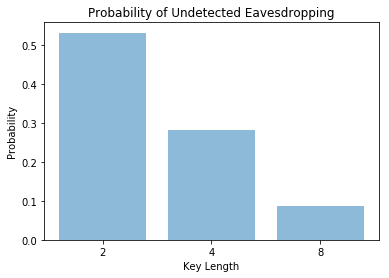
\includegraphics[width=0.5\linewidth]{results.png}	
\caption{Estimated Probability of Eve's interference not being detected in our BB84 simulations using IBM Q Simulator. We estimate probability using the number of occurrences within $2^7$ trials per key length.}
\end{figure}

Hence, we'd expect a probability of undetected eavesdropping of approximately $10^{-128}$ for a 1024-bit key. This shows how rapidly the probability goes to zero. 

Finally, because our simulation excludes a noisy channel and IBM's Q Simulator is error-free in terms of simulating quantum measurements, any time the protocol succeeds a key is exchanged without error. We expect this because both our encoding bases are orthogonal and so if we measure in the correct basis then we should return the correct value, deterministically. In practice, however, Alice's state would be transmitted over a noisy channel and measurements would take place in the presence of interference. Hence, privacy amplification and information reconciliation would be required since Alice and Bob would have correlated but not identical keys after step (8). 

Similarly, if Eve is not eavesdropping then the only reason the protocol can abort is if $b$ and $b'$ agree in less than $2n$ places, given the lack of noisy channel and error-free simulation. This is consistent with what we observed experimentally. 

\subsection{Error bounds of random sampling tests}\label{error_bounds}

Furthermore, we may then ask how likely it is that we find an error below our desired threshold for the check bits when the error would've been found to be above the threshold, had we selected a different subset of $n$ bits. This closely relates to the idea of random sampling tests\cite{text}. 

From the random sample of the $n$ out of our $2n$ bits, we can put an upper bound on the number of errors in the untested bits with high probability. \\

\begin{theorem}\label{thm}
For any $\delta > 0$, the probability of having less than $\delta n$ errors on the $n$ check bits and more than $(\delta+\epsilon)n$ errors on the remaining $n$ bits is asymptotically less than $\exp[-O(\epsilon^2n)]$ for large $n$.

\begin{proof}
\begin{enumerate}
\item Without loss of generality, let $\mu n$ be the total number of errors present in all $2n$ bits, where $0\leq \mu \leq 2$. If there are $\delta n$ errors in the $n$ check bits and $(\delta + \epsilon)n$ errors in the rest of the bits, then $\mu=\delta+(\delta+\epsilon)$, so $\delta =(\mu -\epsilon)/2$. If we have $< \delta n$ errors on the check bits, this means we have $ \geq (\mu -\delta)n$ errors on the rest. \\
Thus, we can prove that our probability $p$ that we have $< \delta n$ errors in the check bits satisfies
$$p<{2n\choose n}^{-1}{\mu n \choose \delta n}{(2-\mu)n \choose (1-\delta)n}\delta n
$$
We show this by assuming the reverse, $p\geq {2n\choose n}^{-1}{\mu n \choose \delta n}{(2-\mu)n \choose (1-\delta)n}\delta n$. We can represent $p$ as
$$p=\sum_{i=0}^{\delta n-1}\frac{{\mu n \choose i}{(2-\mu)n\choose n-i}}{{2n\choose n}}$$
As the probability that we have less than $\delta n$ errors in our check bits is the sum of the probabilities that we get exactly each number between 0 and $\delta n$ errors, and each of these probabilities can be represented as choosing $i$ error bits from the total $\mu n$ errors and $n-i$ clean bits from the rest, divided by the total number of ways which we could choose $n$ bits from $2n$ total. \\
From our assumption earlier, we now have $$\delta n \leq 
\sum_{i=0}^{\delta n-1}\frac{{2n\choose n}^{-1}{\mu n \choose i}{(2-\mu)n\choose n-i}}{{2n\choose n}^{-1}{\mu n \choose \delta n}{(2-\mu)n \choose (1-\delta)n}}$$
Since the left hand side cannot be bigger or equal to the right because of how the binomial probability distribution falls, this cannot be true, so we have a contradiction and our assumption was false. Thus, it is true that 
$$p<{2n\choose n}^{-1}{\mu n \choose \delta n}{(2-\mu)n \choose (1-\delta)n}\delta n
$$
\item For large $n$, we can also bound 
$$\frac{1}{an+1}2^{anH(b/a)}\leq {an \choose bn}\leq 2^{anH(b/a)}
$$
where $H$ is the binary entropy function, $H(p)=-p\log_2p-(1-p)\log_2(1-p)$. So we have 
\begin{align*}
p&<{2n\choose n}^{-1}{\mu n \choose \delta n}{(2-\mu)n \choose (1-\delta)n}\delta n 
\leq 2^{\mu nH(\frac{\delta n}{\mu n})}2^{(2-\mu)nH(\frac{(1-\delta)n}{(2-\mu)n})}(\frac{1} {2n+1}2^{2nH(n/2n)})^{-1}\\
&\leq 2^{\mu n H(\frac{\delta n}{\mu n})}2^{(2-\mu)nH(\frac{(1-\delta)n}{(2-\mu)n})}\frac{2n+1}{2^n}
\end{align*}
\item We know that $H(x)$ is bounded by $H(x)<1-2(x-\frac{1}{2})^2$. We also know that worse case, all the bits are errors, so $\mu=2$, thus
\begin{align*}
p&<2^{\mu n H(\frac{\delta n}{\mu n})}2^{(2-\mu)nH(\frac{(1-\delta)n}{(2-\mu)n})}\frac{2n+1}{2^n}\\
&<2^{2n(1-2(\frac{\delta n}{2n}-\frac{1}{2})^2)}2^{(2-2)n(1-2(\frac{(1-\delta)n}{(2-\mu)n}-\frac{1}{2})^2)}(
\frac{2n+1}{2^n})\\
\end{align*}
We can sub in $\delta=(\mu-\epsilon)/2=(2-\epsilon)/2=1-\frac{\epsilon}{2}$ to get
\begin{align*}
p&<\frac{2n+1}{2^n}2^{2n(1-2(\frac{1-\epsilon/2}{2}-\frac{1}{2})^2)}\\
&<\frac{2n+1}{2^n}2^{2n(1-2(-\frac{\epsilon}{4})^2)}\\
&<\frac{2n+1}{2^n}2^{2n(1-(\frac{\epsilon^2}{8}))}
\end{align*}
Thus we can see that $p<\exp[O(\epsilon^2n)]$, so the probability of getting $< \delta n$ errors in our check bits and $\geq (\delta+\epsilon)n$ errors on the remaining $n$ bits is asymptotically less than $\exp[-O(\epsilon^2n)]$
\end{enumerate}
\end{proof}
\end{theorem}

\section{Conclusion}

In conclusion, we've constructed a robust simulation of the BB84 quantum key exchange protocol using IBM's Q Simulator. Our simulation shows the behavior one would expect with and without the presence of an eavesdropper. Furthermore, to the authors' knowledge, this simulation is the first of its kind---the first demonstration of BB84 using IBM's quantum computation simulators. 

Furthermore, to show the unconditionally secure nature of the algorithm, we derived an error bound for the probability that Eve interferes without the protocol being aborted, which rapidly goes to zero. In our simulations, we found this error bound to be consistent.

We also proved a theorem (Theorem \ref{thm}) that shows that our random sample of check bits used to determine whether to abort the protocol is representative of the complement bits, which are the potential key bits. In particular, the probability that the complementary key bits have greater error than the tested bits decreases in probability at an asymptotically exponential rate. Hence, the check bits used by BB84 are reliable in reflecting Eve's interference. 

We thank Prof. Maggs for providing the opportunity to explore this interesting and rising subtopic of Computer Security. 

\nocite{*}
\bibliographystyle{plain}
\bibliography{course_notes}

\end{document}
